\chapter{Présentation Général de Conception} \label{chap:Présentation Général de Conception}
\section{Introduction}
Dans ce chapitre, nous allons détailler les différentes étapes du processus de conception pour la réalisation de le système proposé .Nous allons également discuter des technologies et des outils disponibles. Ansi nous avons divisé ce chapitre en deux phases. Dans la première phase qui intitulée la conception Hardware et la deuxième est Software.
\section{Conception Hardware}
Des dispositifs ou outils physiques utilisés dans le processus de conception et de réalisation du prototype proposé, ainsi que les matériels informatiques et autres dispositifs électroniques , se présente comme se qui suit.

\subsection{Prototype de Système}
Sur la base de l’étude des composants et le besoin fonctionnel de notre projet, présentée dans les chapitres précédents, on a put sélectionner les déférents composants (capteurs,..) et leur liaison avec ESP8266 (i.e. figure 3.1), qui va collecter les information provenant de ces capteurs a fin de les analyser et de réagir par conséquence  aux événements en donnant des ordres au déférents composants électrique en temps réel. Tous les données et ordres enregistrés sont en suite envoyer à la machine relié au contrôleur  système, par le biais un réseau local. Le système qui se trouve sur cette machine, (i.e. conception software)   va les stocker et les analyser pour une future exploitation, par une machine Learning, pour une utilisation rationnelle de la serre. 
\begin{figure}[hbt]
\right
\label{fig:Prototype}

 \fcolorbox{black}{white}{ 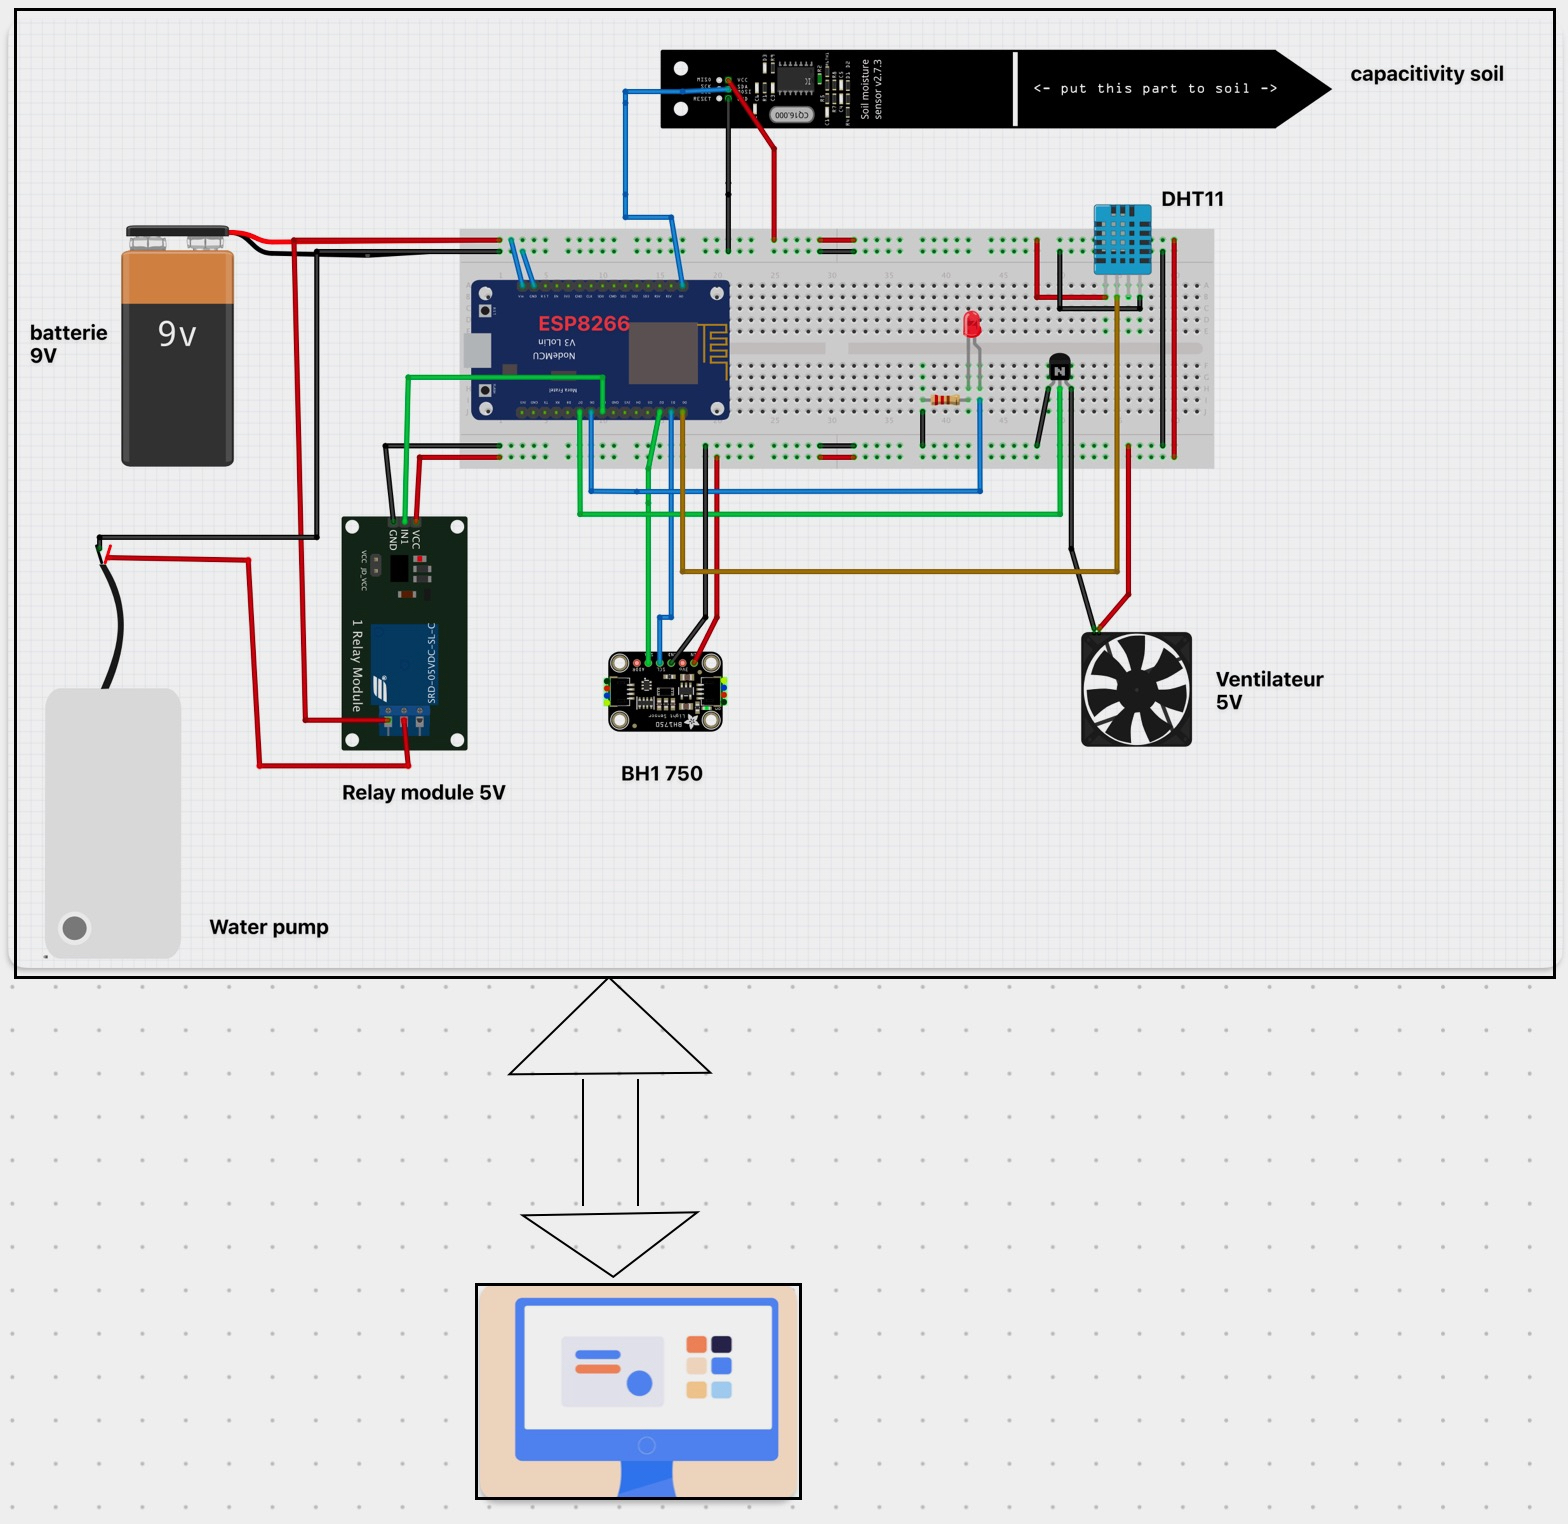
\includegraphics[width=18cm]{figures/prototype.jpg}}\caption{Protoype}
\end{figure}
\newline

\section{Conception Software}
\textbf{ La conception de logiciels}  est un processus critique pour le développement de logiciels efficaces, sûrs et fonctionnels. Elle implique l'élaboration de la structure, de l'architecture et de la fonctionnalité du logiciel.
Notre projet, comme  le montre dans le schéma de principe Hardware (i.e. Figure 3.1)et l`architecture globale du systeme (i.e Figure 3.2 ) \newline prévoit deux parties de conception software à savoir : 
\newline
\textbf{La conception software du micro contrôleur ESP8266} qui, selon la description fonctionnel de notre projet présenté dans la section 3.3.1, à pour rôle de (i.e.  future figure 3.3):
	\newline
   - Capter les paramètres de configuration provenant de la machine reliée au micro-contrôleur ESP8266 .
\newline
	- Capter périodiquement les événements provenant des capteurs .
\newline
	- Analyser ces événements et de réagir selon leurs situation .
	\newline
	- Informer la machine reliée au micro contrôleur ESP8266 de tout événement.
\newline
	\textbf{La conception software du système} se trouve sur la machine relié au micro contrôleur ESP8266, qui selon les besoins fonctionnel de notre projet, présenté dans la section 3.3.2 à pour rôle de stocker/analyseur d’information enregistré par le contrôleur et qui se résume par :
	\newline
	- Capter les paramètres, ou information en provenance de l’utilisateur Humain par l’interface Humain .
	\newline
	- Informer le micro contrôleur ESP8266 de tout changement de paramètres par le biais de l’interface réseau .
	\newline
	- Capter les informations en provenance du micro contrôleur ESP8266, par le biais de l’interface réseau .
	\newline
	- Stocker toute les informations en provenance de l’utilisateur Humain et/ou le micro contrôleur ESP8266 .
	\newline
	- Analyser toute ces informations et informer l’utilisateur Humain par l’interface Humain sous la forme d’un tableau de bore décisionnel. 
	
\newpage
\subsection{Architecture global du système}
Sur la base de cette description fonctionnelle des rôles des deux parties software, l’architecture globale de notre prototype est comme indiqué sur la Figure suivante : 
\begin{figure}[hbt]
\centering
\right

\label{fig:Architecture global du système}
\fcolorbox{black}{white}{ 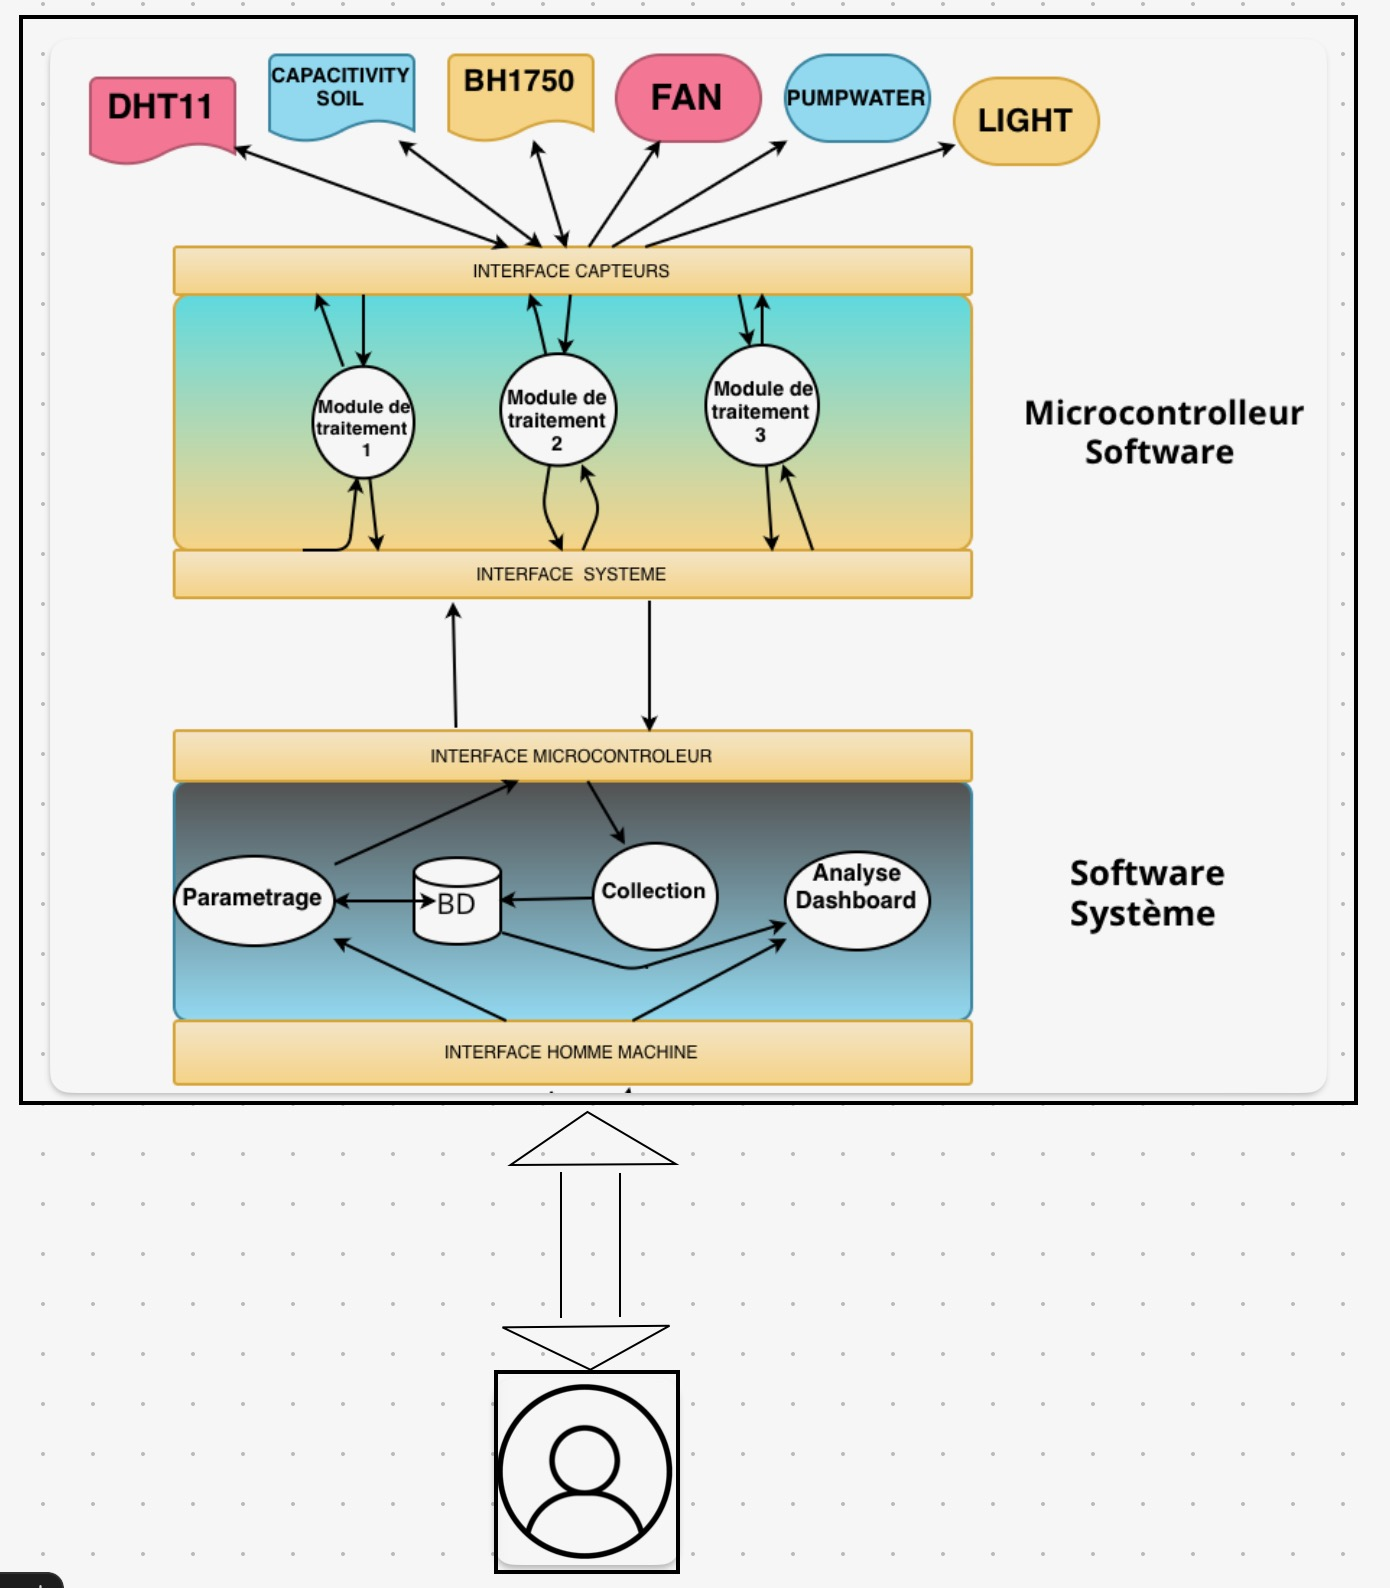
\includegraphics[width=14cm]{figures/1.jpeg}}
\caption{Architecture global du système}
\end{figure}

\newpage
\subsection{L’architecture Software du Micro-contrôleur}
La décomposition de l’architecture Software du micro contrôleur ESP8266 est comme indiqué sur la Figure suivante : 
\begin{figure}[hbt]
\centering
\right
\label{fig:Architecture Software Micro-Controlleur}
\fcolorbox{black}{white}{ 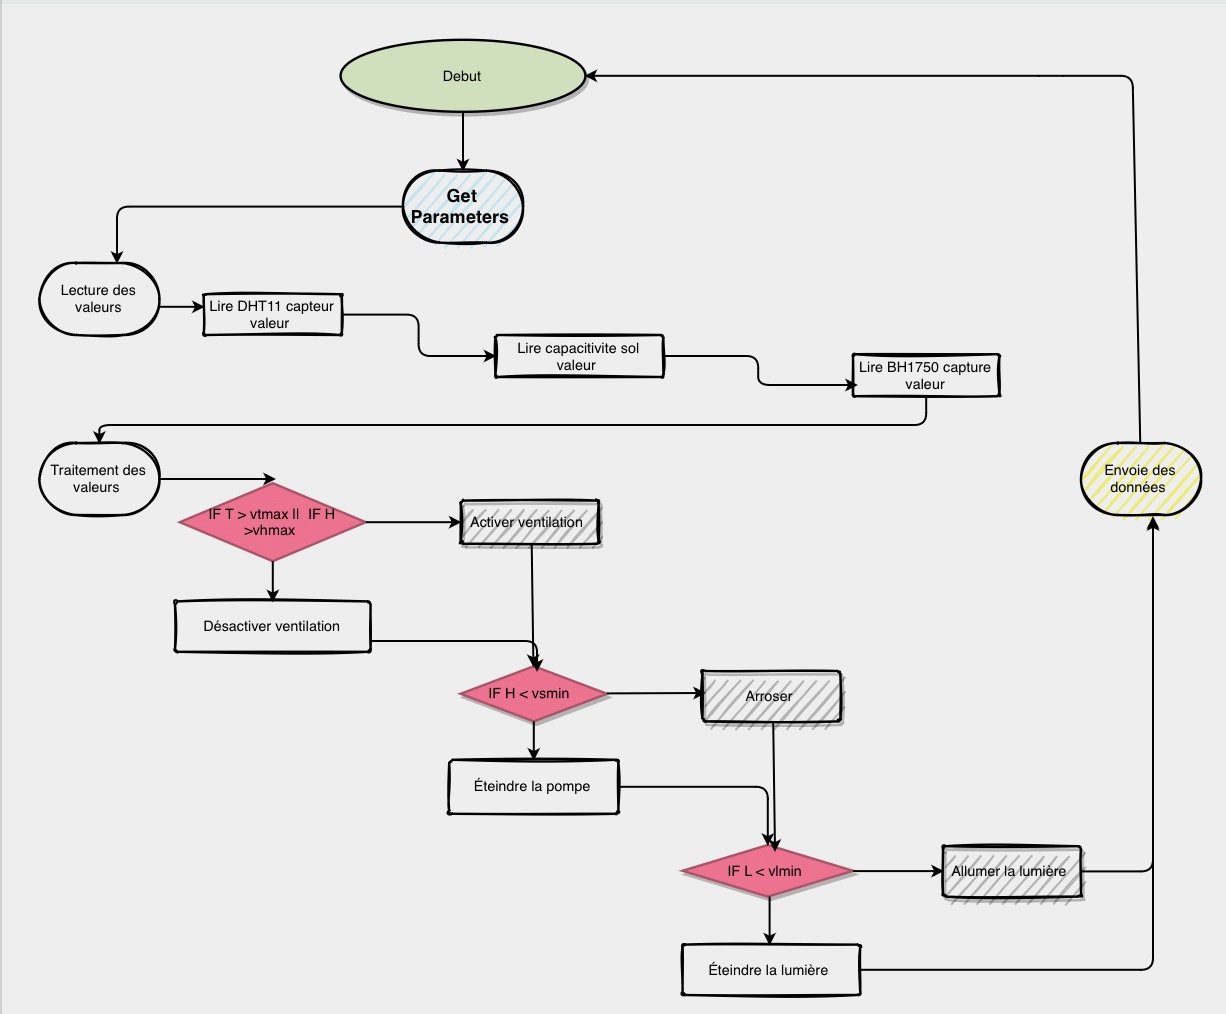
\includegraphics[width=18cm]{figures/agm.jpeg}}
\caption{Architecture Software Micro-Controller}
\end{figure}


\newpage
\subsection{L’architecture Software du Stockeur/Analyseur }
La décomposition de l’architecture Software du Système Stockeur/Analyseur des événements enregistrés est comme indiqué sur la Figure prochaine :

\begin{figure}[hbt]
\centering
\right
\label{fig:L’architecture Software du Stockeur/Analyseur }

 \fcolorbox{black}{white}{ 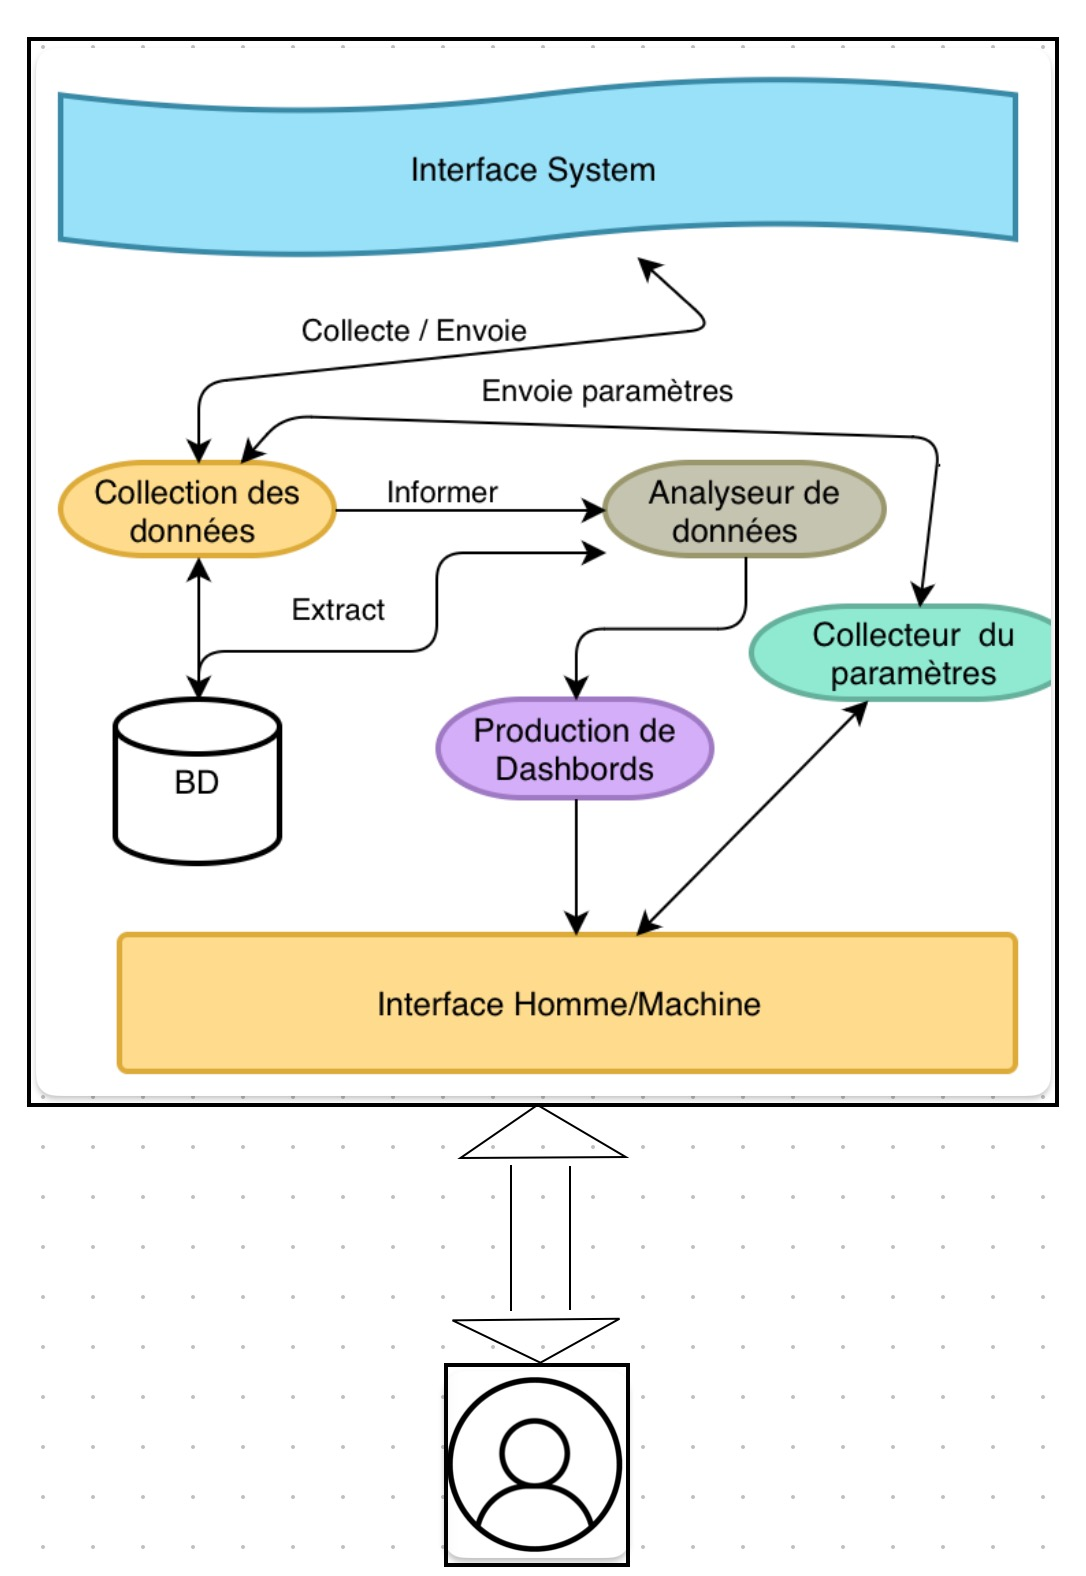
\includegraphics[width=11cm]{figures/2.jpeg}}\caption{L’architecture Software du Stockeur/Analyseur }
\end{figure}

\newline
Il convient de noter que la conception du système est un processus complexe et nous serons la détailler par diagramme de classe et des diagrammes de séquence pour bien comprendre.
\newpage
\section{Diagramme de séquence}
Les diagrammes de séquences permettent de décrire comment les éléments du système interagissent entre eux et avec les acteurs. Diagramme de séquence est d’identifiez les objets et les acteurs, déterminez l'ordre des interactions, ajoutez les messages, incluez les conditions et les boucles. Il permet de comprendre comment les objets collaborent pour réaliser une fonctionnalité ou un processus donné. 

\subsection{Diagramme de séquence Micro-Controleur}
\begin{figure}[hbt]
\centering
\right
\label{fig: DS Micro-Controleur}

  \fcolorbox{black}{white}{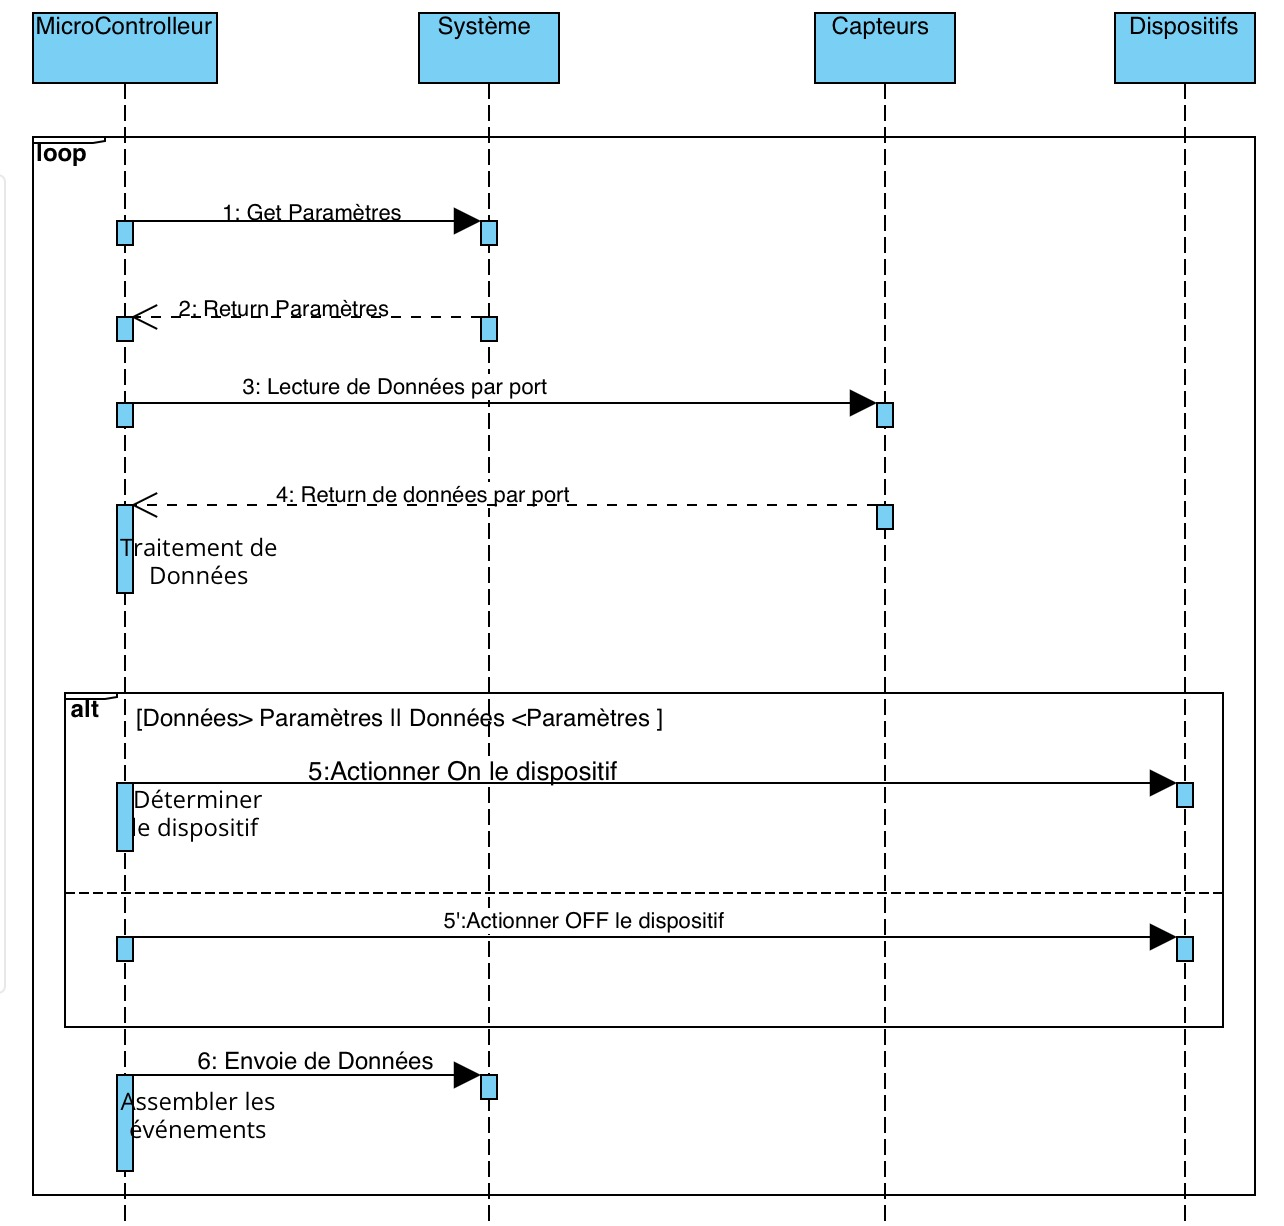
\includegraphics[width=15cm]{figures/microcontroller.jpeg}}
  \caption{Diagramme de séquence Micro-Controleur}
\end{figure}


\break
\subsection{Diagramme de séquence Dashboard Des Évènements }
\begin{figure}[hbt]
\centering
\right
\label{fig: DS Dashboard Des Évènements}

  \fcolorbox{black}{white}{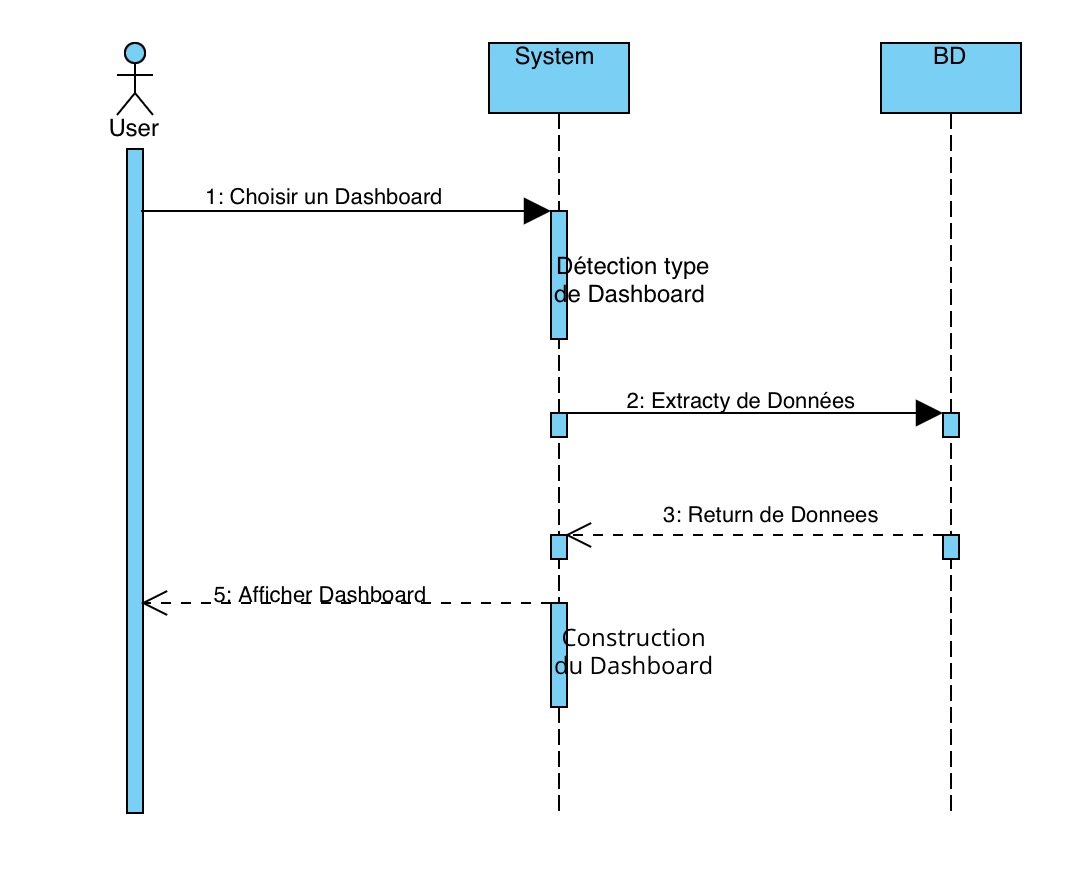
\includegraphics[width=15cm]{figures/dashboardev.jpeg}}
  \caption{Diagramme de séquence Dashboard Des Évènements}
\end{figure}

\break
\subsection{Diagramme de séquence Dashboard Des décisions }
\begin{figure}[hbt]
\centering
\right
\label{fig: DS Dashboard Des décisions }
  \fcolorbox{black}{white}{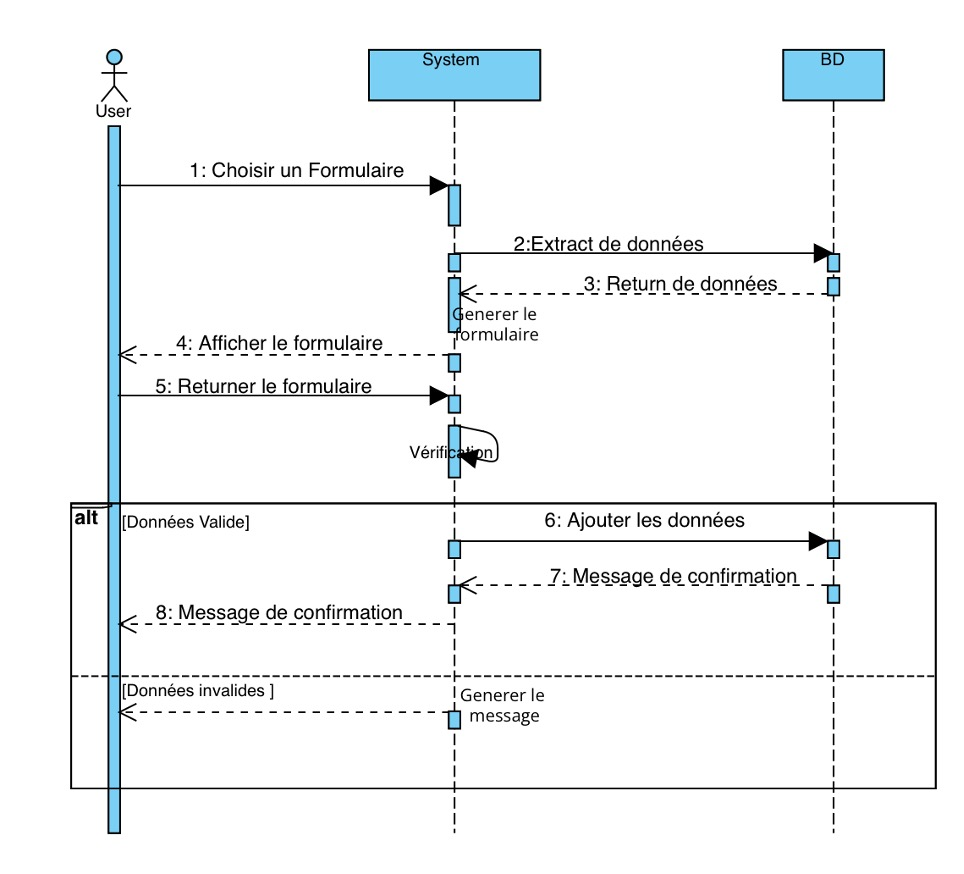
\includegraphics[width=15cm]{figures/dsD.jpg}}
  \caption{Diagramme de séquence Dashboard Des décisions }
\end{figure}

\newpage
\section{Diagramme de classes}
Un diagramme de classes est un type de diagramme de modélisation qui représente les classes et les relations entre les classes. Il est utilisé dans la modélisation orientée objet pour visualiser la structure statique d'un système :les classes, les attributs, les opérations et les relations entre les classes. Notre diagramme du système  figure prochaine :


\begin{figure}[hbt]
\centering
\right
\label{fig:Diagramme de classe}

 \fcolorbox{black}{white}{ 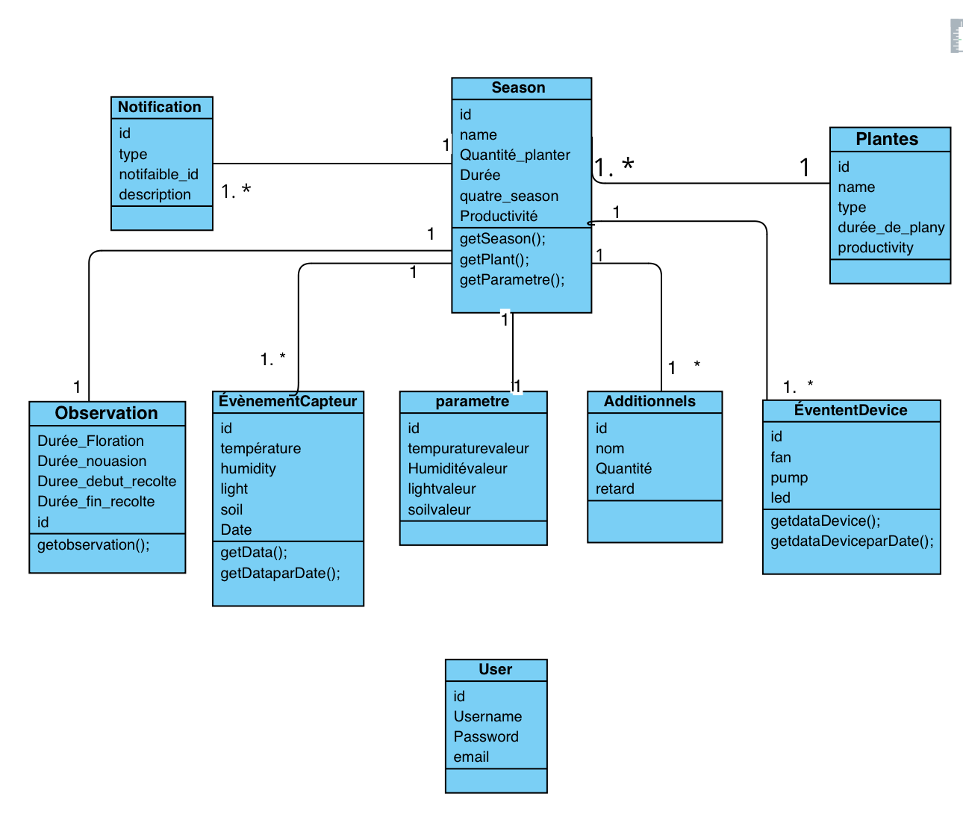
\includegraphics[width=18cm]{figures/diagrammeclass.png}}
 \caption{Diagramme de classe}
\end{figure}

\newpage
\section{Shéma de BD}
\newline

\begin{figure}[hbt]
\centering

\label{fig:Shema BD}

 \fcolorbox{black}{white}{ 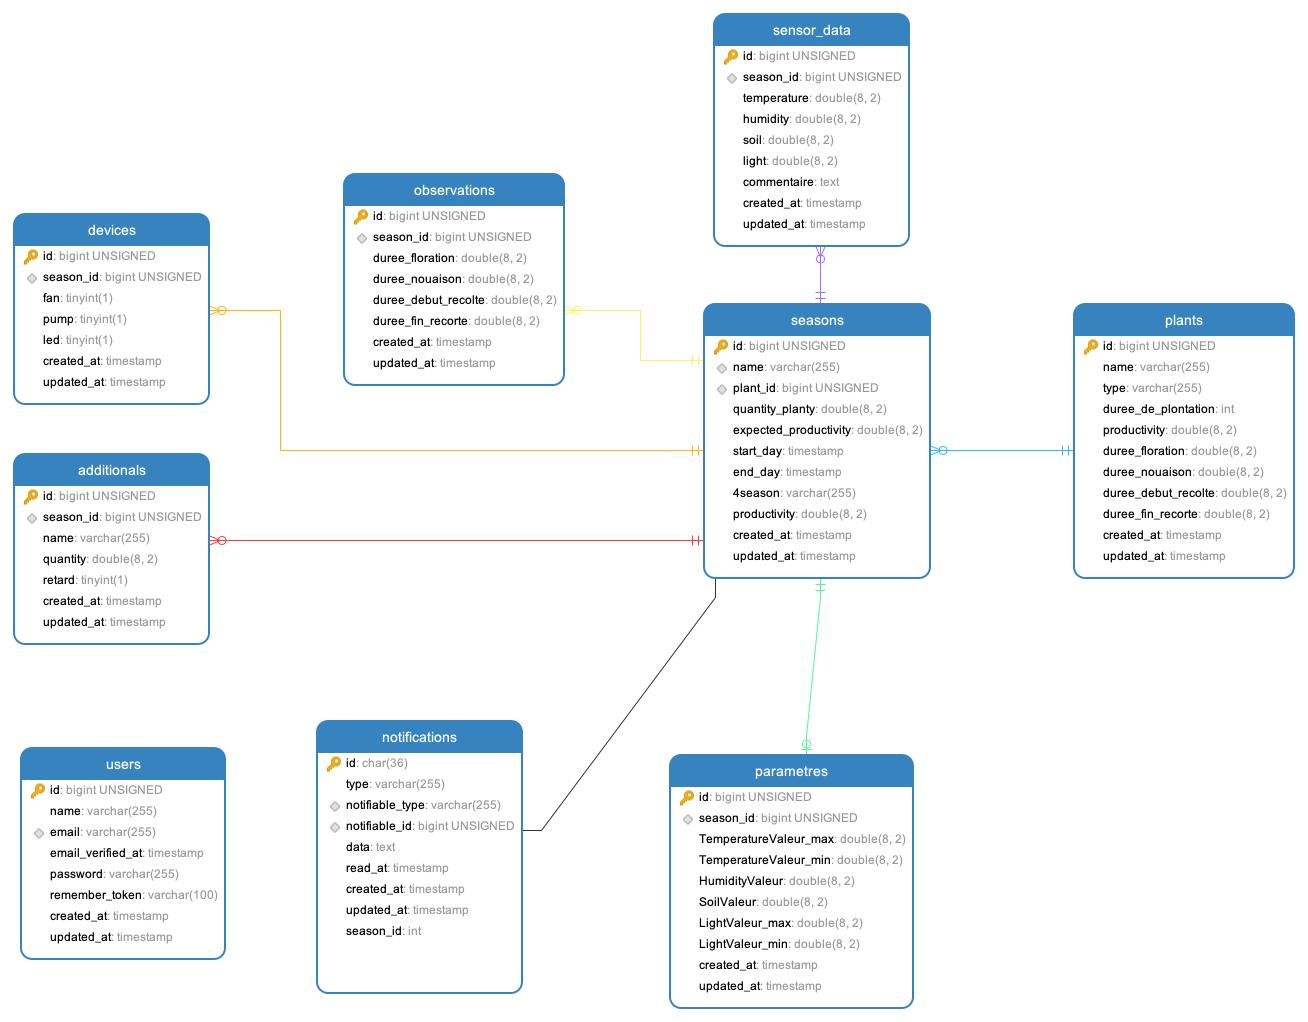
\includegraphics[width=18cm]{figures/SHEMABD.jpg}}
 \caption{Shema BD}
\end{figure}

\break
\section{Conclusion}
Ce chapitre a couvert tous les détails structurels du système. On début , nous avons expliqué l'architecture globale du système et le principe de la solution . Ensuite, nous sommet entré dans les détails de chaque partie et nous avons
fourni tout ce qui concernait la système .
Dans le chapitre suivant, En décrire les résultats du projet, nous décrivons également l'organigramme et les technologie utiliser
dans le système.
 